\chapter{Background} \label{background}

In this chapter, I summarize the related background to this thesis. I briefly present formal methods and model checking (\autoref{sec:form-methods}), and formal models of different abstraction levels (\autoref{sec:form-models}). I also present the need for simulation (\autoref{sec:sim}) and the tools related to my work (\autoref{sec:tools}).

\section{Formal Methods}\label{sec:form-methods}

\textit{Formal methods} are precise approaches for the analysis of systems. They rely on mathematical logic, therefore they can be used only on mathematically precise \textit{formal models}. They are widely used for verification purposes in safety-critical domains (e.g., automotive, railway, and aerospace industries) where it is crucial to guarantee the safety of systems.

\subsection{Model Checking}

\textit{Model checking}~\cite{mc} is a formal method for the algorithmic analysis of the dynamic behavior of systems, checking whether a system satisfies a given requirement or not. The high-level overview of model checking is shown in \autoref{fig:mc}.

To apply model checking, three building blocks are required~\cite{IntroductionToModelChecking}:
\begin{itemize}
    \item \textit{Formal model}: A mathematically precise model of the behavior of the system is required, usually a \textit{transition system}~\cite{IntroductionToModelChecking}.
    \item \textit{Formal requirement}: The verifiable requirement should also be in a mathematically precise form, for which \textit{temporal logic}~\cite{tl} is appropriate.
    \item \textit{Algorithm}: Finally, an (effective) algorithm is required to decide whether the given formal model satisfies the given formal requirement or not. The output of the algorithm is a \textit{proof} or a \textit{counterexample}.
\end{itemize}

\begin{figure}[htbp]
\centering
\includesvg[inkscapelatex=false, width=0.9\textwidth, keepaspectratio]{figures/mc.svg}
\caption{Model checking.}
\label{fig:mc}
\end{figure}

Although with traditional \textit{testing} bugs can be found in systems, the correctness of a system can not be \textit{proved}. Model checking explores the entire state space of the system, making it possible to mathematically \textit{prove} that the system satisfies a certain requirement.

\section{Formal Models}\label{sec:form-models}

As systems -- especially safety-critical systems -- are becoming more complex, new development approaches, such as \textit{model-based systems engineering} (MBSE)~\cite{mbse}, have been introduced to handle complexity. In MBSE, models are the primary artifacts of the development process.~\cite{Seidewitz2003} To create these models, suitable modeling languages are required to model the different aspects of systems, e.g., structure or behavior.

In the case of \textit{behavioral models}, it is especially important to have precise formal semantics in order to be able to \textit{execute} them -- either by directly simulating them or by automatically transforming them into an executable formalism, e.g., program code.

\subsection{Component-Based Reactive Systems}

\textit{Component-based} development is a practical approach in the case of complex systems: engineers can compose such systems from reusable parts (\textit{components}) which are communicating with each other through well-defined interfaces.

\textit{Reactive} systems are interacting with their environment. These interactions are modeled as input and output events: input events coming from the environment can trigger internal behaviors (e.g., state change) of the system (i.e., the system \textit{reacts} to an event), while the system can react with output events to its environment. The possible interactions between the system and its environment can also be modeled with interfaces.

In the case of \textit{component-based reactive systems}, the components of the system can be modeled as \textit{state machines}~\cite{Gamma}. Informally, a state machine is a reactive component, because its behavior is modeled as \textit{transitions}, triggered by input events and generating output events.

\textit{State machines} are state-based models, focusing on the internal state of the system, and the transitions changing it. This modeling approach can be used at different abstraction levels. \textit{Finite state machine} (\autoref{ssec:fsm}) is a low-level mathematical, while \textit{Statechart} (\autoref{ssec:statechart}) is a high-level engineering formalism.

\subsection{Mathematical Finite State Machine}\label{ssec:fsm}

\textit{Finite state machine} is a mathematical formalism to model the state-based behavior of a system. Informally, it defines the possible states and state changes (\textit{transitions}) of a system. It can be either \textit{deterministic} or \textit{non-deterministic}, according to the number of possible transitions at a specific state, triggered by a specific input event.

\begin{definition}[Finite State Machine]\label{def:fsm}
    Formally, a deterministic finite state machine is a 5-tuple $SM = \langle S, s_0, I, O, T \rangle$ where:
    \begin{itemize}
        \item $S = \{ s_1, s_2, \ldots, s_n  \}$ is a finite set of \textit{states}.
        \item $s_0 \in S$ is the \textit{initial state}.
        \item $I = \{ i_1, i_2, \ldots, i_m \}$ is a finite set of \textit{input events} coming from the environment.
        \item $O = \{ o_1, o_2, \ldots, o_l \}$ is a finite set of \textit{output events} going to the environment. Note, that $I$ and $O$ are disjoint, i.e., $I \cap O = \emptyset$.
        \item $T: (I \times S) \mapsto (S \times O)$ is the (fully defined) \textit{transition function}, representing the reaction of the state machine to a specific input event in a specific state, i.e., the new state and the generated output event.
    \end{itemize}
\end{definition}

In Definition \ref{def:fsm}, I define a fully-defined deterministic finite state machine, i.e., which can take exactly one transition at every state, reacting to every input event. Note, that this does not mean, that the system must always change its state because a transition can lead the system to the same state as it was already in. The lack of the generated output event can be modeled with a special output event $\varepsilon$, i.e., a transition $T(i, s) = (s, \varepsilon)$ means that the system does not react to input event $i$ in state $s$.

Note, that the determinism of the state machine only means that the state machine itself is deterministic. Nevertheless, it can be used to model a system with a non-deterministic environment, by non-deterministically choosing the input events of the state machine.

\begin{example}[Finite State Machine]\label{ex:fsm}
    Consider a machine with two buttons, \emph{do} and \emph{reset}, which beeps after every third press of button \emph{do}, while the press of button \emph{reset} resets the counter. This machine can be modeled with the following deterministic finite state machine $SM = \langle S, s_0, I, O, T \rangle$:
    \begin{itemize}
        \item $S = \{ s_0, s_1, s_2  \}$ where $s_n$ represents the state where $n$ \emph{do} presses are counted since the last \emph{beep} or \emph{reset} press.
        \item $s_0 \in S$ is the \textit{initial state}.
        \item $I = \{ do, reset \}$ where the button presses are modeled as \textit{input events}.
        \item $O = \{ beep, \varepsilon \}$ where $beep$ models the beep of the machine as an \textit{output events}, and $\varepsilon$ models the lack of beep.
        \item $T =
        \begin{Bmatrix}
        (&do,& s_0,& s_1,& \varepsilon&),\\
        (&do,& s_1,& s_2,& \varepsilon&),\\
        (&do,& s_2,& s_0,& beep&),\\
        (&reset,& s_0,& s_0,& \varepsilon&),\\
        (&reset,& s_1,& s_0,& \varepsilon&),\\
        (&reset,& s_2,& s_0,& \varepsilon&)
        \end{Bmatrix}$
    \end{itemize}

    The transition function can be represented as a \emph{state-transition table}. Each cell represents the effect of the given input event in the given state as a pair of the next state and the output event.

    \begin{table}[htbp]
    \centering
    \begin{tabular}{|c||c|c|c|}
     \hline
     State/Input & $s_0$ & $s_1$ & $s_2$ \\
     \hline\hline
     $do$ & ($s_1$, $\varepsilon$) & ($s_2$, $\varepsilon$) & ($s_0$, $beep$) \\ 
     \hline
     $reset$ & ($s_0$, $\varepsilon$) & ($s_0$, $\varepsilon$) & ($s_0$, $\varepsilon$) \\
     \hline
    \end{tabular}
    %\caption{The state-transition table of finite state machine defined in \autoref{ex:fsm}.
    \label{tbl:stt}
    \end{table}

    The state machine can also be represented graphically as a graph. The nodes represent the states, while the edges represent the transitions. An edge with label $i / o$ represents a transition leading the system from the state represented by the source node to the state represented by the target node, triggered by input event $i$, producing output event $o$.

    \begin{figure}[htbp]
    \centering
    \includesvg[inkscapelatex=false, width=0.5\textwidth, keepaspectratio]{figures/fsm.svg}
    \caption{Graphical representation of the example finite state machine.}
    \label{fig:fsm}
    \end{figure}
    
\end{example}

\subsection{High-Level Statechart}\label{ssec:statechart}

The \textit{statechart} formalism is a popular tool to model the behavior of state-based reactive systems in a higher abstraction level~\cite{Harel}. It relies on the mathematical \textit{finite state machine} formalism but it is more expressive, making the formalism usable in everyday engineering work.

In general, the statechart formalism extends the finite state machine formalism with the following:
\begin{itemize}
    \item \textit{Hierarchically nested states}: The internal behavior of a state (\textit{superstate}) can be modeled with an inner statechart (\textit{substates}). The inner statechart operates in the context of the superstate. When the superstate is activated, its initial inner state activates, too. When the superstate is deactivated, its whole inner statechart deactivates.
    \item \textit{Orthogonal regions}: The internal behavior of a state can be modeled with several statecharts (\textit{regions}), running independently.
    \item \textit{Entry and exit actions}: Like in the case of transitions, \textit{entry} and \textit{exit} actions can be defined for states. These actions are triggered when the state is activated or deactivated, respectively.
\end{itemize}

\begin{example}[Statechart]\label{ex:sch}
    Consider the extension of the finite state machine defined in Example \ref{ex:fsm}. A new input event \emph{switch} is introduced to switch the whole machine on/off. When the machine is switched on/off, it beeps. When the machine is turned on, it beeps when the reset button is pressed first since the machine is turned on.

    It serves as an example for all of the three new features of the statechart formalism. The initial \emph{Off} state defines an entry and exit action for beeping. The hierarchical \emph{On} state contains two orthogonal regions which are independently responsible for counting the \emph{do} and \emph{reset} events.

    The graphical representation of this statechart is shown below.

    \begin{figure}[htbp]
    \centering
    \includesvg[inkscapelatex=false, width=0.8\textwidth, keepaspectratio]{figures/sch.svg}
    \caption{Graphical representation of the example statechart.}
    \label{fig:sch}
    \end{figure}
    
\end{example}

The statechart formalism can be further extended, e.g. with \textit{variables} and \textit{guards}. Guards on transitions are logical expressions over variables, and a transition can not be fired if its guard evaluates to false.

The informally introduced high-level formalism has several concrete definitions in different modeling languages such as the general-purpose \textit{Unified Modeling Language}(UML)~\cite{uml} and \textit{Systems Modeling Language} (SysML)~\cite{sysml} developed by the \textit{Object Management Group} (OMG), though these formalisms often lack precise formal semantics~\cite{Elekes2022}.

\subsubsection{Non-Determinism}

The execution of a statechart can be non-deterministic due to several reasons. In general, we distinguish two types of non-determinism: \textit{internal} and \textit{external}.

\paragraph{Internal non-determinism.} A single step of a statechart can contain non-deterministic decision point(s). This means, that in a specific state configuration, with a specific input event, the statechart can behave in different ways. Due to the fact, that the environment can only interact with the statechart with input events (i.e., the statechart itself is a \textit{black box} in terms of control), internal non-determinism makes the behavior of the system uncontrollable, causing problems in several use cases, e.g., precise simulation.

The systematic analysis of (internal) non-determinism in statechart semantics is beyond the scope of this work, here I only highlight some examples to underline its necessity.

\begin{itemize}
    \item \textit{Multiple fireable transitions}: In real-life engineering work, especially with the growing complexity of state hierarchies and guard expressions, statecharts are usually not deterministic and fully defined. This means, that in a specific state configuration, an input event may trigger multiple transitions. Although state machine semantics usually define some rules to select the transition to fire, in some cases neither of these rules defines the \textit{exact} transition(s) to fire, i.e., the choice from the firable transitions remains non-deterministic.
    \item \textit{Orthogonal regions}: The execution of orthogonal regions is independent, meaning that there is no guarantee on the order of their steps. As a result, the exact ordering is non-deterministic.
    \item \textit{Composition}: Individual statecharts usually serve as components of a more complex system. In this case, the composition of the statecharts may not define their exact execution order, causing non-determinism, too.
    %\item \textit{Environment}: The environment of statecharts is usually modeled using non-determinism to cover the possible inputs. This kind of non-determinism is intentional, making it necessary to select the actual environment behavior during execution explicitly.
\end{itemize}

\paragraph{External non-determinism.} An obvious source of non-determinism during execution is the behavior of the \textit{environment}, i.e., the input events sent to the statechart. This is called external non-determinism, and does not cause problems like internal non-determinism. External non-determinism is observable and controllable, e.g., during simulation, it is typically handled by the user of the simulator by ``impersonating`` the environment, i.e., choosing the next event to send (and its parameters, if any).


\subsection{Extended Symbolic Transition System}\label{ssec:xsts}

Extended Symbolic Transition System (XSTS)~\cite{XSTS} is a suitable low-level formalism to describe higher-level (reactive) systems, such as statecharts. Informally, an XSTS model describes variables and transition sets, and in every step a non-deterministically selected atomic transition fires from the appropriate transition set. In this thesis, I introduce XSTS based on my previous work~\cite{xsts-split}.

\begin{definition}[Extended Symbolic Transition System]
Formally, an XSTS model is a 4-tuple $XSTS = \langle V, Tr, In, En \rangle$ where:
\begin{itemize}
    \item $V = \{ v_1, v_2, \ldots, v_n  \}$ is a set of \textit{variables} with domains $D_{v_1}, D_{v_2}, \ldots, D_{v_n}$, e.g. \emph{integer}, \emph{bool}, or \emph{enum}. An \emph{enum} domain is just syntax sugar, a set of \emph{literals} which are different values with a textual representation.
    \item A state of the system is $s \in S \subseteq D_{v_1} \times D_{v_2} \times \cdots \times D_{v_n}$, which can be regarded as a value assignment: $s(v) \in D_v$ for every variable $v \in V$.
    \item $Tr \subseteq S \times S$ is the \textit{internal transition relation}, describing the behaviour of the system itself;
    \item $In \subseteq S \times S$ is the \textit{initial transition relation}, describing the initialization of the system, which is executed only once at the beginning of the execution;
    \item $En \subseteq S \times S$ is the \textit{environmental transition relation}, describing the environment which the system is interacting with;
    \item Both $Tr$, $In$, and $En$ may be defined as a union of individual transitions that the system can take. Abusing the notation, we will denote these transitions as $t \in Tr$ which actually means that $t \subseteq S \times S$ as a transition relation is a subset of $Tr$.
\end{itemize}
\end{definition}

A \textit{concrete state} of the system is $c \in C = D_{v_1} \times D_{v_2} \times \cdots \times D_{v_n}$, which is a value assignment $c: v \mapsto c(v) \in D_v$ for every variable $v \in V$. A concrete state $c$ can also be described with a logical formula $\varphi = (v_1 = c(v_1) \wedge \cdots \wedge v_n = c(v_n))$ where $\mathrm{var}(\varphi) = V$.
%A concrete state $c$ can also be described with a logical formula $\varphi$ where $var(\varphi) \subseteq V$ or $var(\varphi) = V$ if $\top \in D_v$ for every $v \in V$ where $v = \top$ means there is no restriction on the value of $v$ so it can be anything from $D_v$.

%= 2^{D_{v_1}} \times 2^{D_{v_2}} \times \cdots \times 2^{D_{v_n}}$
An \textit{abstract state} of the system $s \in S = 2^C$ may cover more concrete states $s = \{ c_1, \ldots, c_m \}$. We use the notation $0 \leq |s| \leq 2^{|C|}$ for the number of concrete states covered by abstract state $s$. Like in the case of concrete states, the notation $s(v) = x$ where $x \in D_v$ means that $c(v) = x$ in every concrete state $c \in s$ covered by $s$.
%If there is no restriction on variable $v$, i.e. it can have any value from $D_v$, we use the notation $s(v) = \top$.
The logical formula of an abstract state is $\varphi = ((v_1 = c_1(v_1) \wedge \cdots \wedge v_n = c_1(v_n)) \vee \cdots \vee (v_1 = c_m(v_1) \wedge \cdots \wedge v_n = c_m(v_n)))$ where $\mathrm{var}(\varphi) = V$, and it covers exactly $m$ (maybe infinite) concrete states.

Note, that every concrete state $c$ is also an abstract state $s$ covering only 1 concrete state $c$, so $|c| = |s| = 1$. Thus, without the loss of generality, we use abstract states in the following even without explicitly stating that a state is abstract.

Each transition relation $T \in \{ Tr, In, En \}$ is a set of transitions $t$ where a transition leads the system from a state $s$ to a successor states $s'$: $T \subseteq \{ t=(s, s') \in S \times S \}$.

Every domain $D$ has an initial value $IV(D) \in D$ e.g., $IV(\textit{bool}) = \textit{false}$, $IV(\textit{integer}) = 0$. Every variable $v$ can have a custom initial value $IV(v) \in D_v$ but it is not necessary, because its domain $D_v$ always has one. The only (concrete) \emph{initial state} $s_0$ is given as the \emph{initial value} for each variable $v$: $s_0(v) = IV(v)$ if $IV(v)$ exists, otherwise $s_0(v) = IV(D_v)$. The execution of the system starts with assigning the initial value $s_0(v)$ to every variable $v \in V$.

From the initial state $s_0$, $In$ is executed exactly once. Then, $En$ and $Tr$ are executed in alternation. In state $s$, the execution of a transition relation $T$ (being either of the transition relations) means the execution of exactly one non-deterministically selected $t \in T$ transition. Transition $t$ is enabled if $t(s) \neq \emptyset$. If a transition is not enabled, it can not be executed. If $\forall t \in T: t(s) = \emptyset$, transition relation $T$ can not be executed in state $s$, and therefore $s$ is a deadlock. In addition to the non-deterministic selection, transitions may be non-deterministic internally, therefore even in the case of a concrete state $c$, $t(c) = \{c^\prime_1, \ldots, c^\prime_k\}$ may yield a set of successor concrete states. In other words, in the case of a general transition $t=(s, s^\prime)$, there is no restriction on the relation between $|s|$ and $|s^\prime|$.

\subsubsection{XSTS Operations}\label{ssec:xsts-ops}
Transitions are described as $op \in Ops$ \textit{operations}, which may be atomic or composite operations. The semantics of transitions are defined through the semantics of operations, which is, in turn, the definition of $op$ as a relation over $S \times S$. For a precise description, refer to~\cite{XSTS} -- for this work, an informal definition is sufficient.

XSTS defines the following \emph{basic operations} which lead the system from state $s$ to successor state $s^\prime$:
    \begin{itemize}
        \item \textit{Assignments}: An assignment of form $v := \varphi$ with $v \in V$ and $\varphi$ as an expression of the same type $D_v$ means that $\varphi$ is assigned to $v$ in the successor state $s^\prime$ and all other variables keep their value. Formally, $s^\prime = \bigcup c^\prime$, where $c^\prime(v) = \varphi \wedge c^\prime(v^\prime) = c(v^\prime)$ for every $v^\prime \neq v \in V$ and every $c \in s$. Therefore, the number of concrete states covered by $s^\prime$ is less than or equal to the number of concrete states covered by $s$: $|s^\prime| \leq |s|$.
        \item \textit{Assumptions}: An assumption of form $[\psi]$ with $\psi$ as a Boolean expression over the variables ($\mathrm{var}(\psi) \subseteq V$) checks condition $\psi$ without modifying any variable and can only be executed if $\psi$ evaluates to \textit{true} over the current state $s$, i.e., over at least one concrete state $c \in s$. In this case, the successor state $s^\prime$ covers the concrete states $c \in s$ covered by the original state $s$ where $\psi$ evaluates to \textit{true}, therefore $|s^\prime| \leq |s|$. Otherwise, i.e., when $\psi$ evaluates to \textit{false} over every concrete state $c \in s$, the set of successor states is the empty set $\emptyset$, and $|s^\prime| = 0$.
        \item \textit{Havocs}: A havoc of form $\havoc(v)$ with $v \in V$ means a non-deterministic assignment to variable $v$, i.e., after execution, the value of $v$ can be anything from $D_v$ and all other variables keep their value. Formally, $s^\prime = \bigcup_{c \in s} \{ c^\prime_1, \ldots, c^\prime_{|D_v|} \}$, where $c^\prime_i(v) = D_{v_i} \wedge c^\prime_i(v^\prime) = c_i(v^\prime)$ for every $v^\prime \neq v \in V$ where $D_v = \{ v_1, \ldots, v_{|D_v|} \}$. Therefore, $|s^\prime| \geq |s|$.
        \item \textit{Local variables}: A local variable can be declared as an operation of form $\mathit{var}\ v_{\mathit{\mathrm{loc}}} : \mathit{type} :=\varphi$.\footnote{The default value of the type is used as an initializer unless explicitly specified by the modeler.} A local variable can only be accessed in its \textit{scope} which is its direct container composite operation. Technically, the declaration of a local variable $v_{\mathrm{loc}}$ adds it to $V$ and assigns its initial value $\varphi$ to $v_{\mathrm{loc}}$ while the end of every scope removes every local variable declared in it from $V$. Thus, local variables increase the state space \textit{only} inside their container transitions. Due to the atomicity of transitions, local variables do not modify the state space of the system itself. Formally, $V^\prime = V \cup \{ v_{\mathrm{loc}} \}$, $s^\prime(v_{\mathrm{loc}}) = \varphi$, $s^\prime(v) = s(v)$ for every $v \in V$, and $|s^\prime| = |s|$.
    \end{itemize}
\emph{Composite operations} contain other operations but their execution is still atomic. Practically, this means that the contained operations are defined over transient states and the composite operation determines which one(s) will be the (stable) result of the composite operation. XSTS defines the following composite operations:
    \begin{itemize}
        \item \textit{Sequences}: A sequence of form $op_1, \ldots, op_n$ is composed of operations $op_1, \ldots, op_n$ with $op_i \in Ops$ executed sequentially, each applied on every successor state of the previous one (if any). The successor state after executing the sequence is the result of the last operation.
        Each operation $op_{i+1}=(s_{i+1}, s^\prime_{i+1})=(s^\prime_{i}, s^\prime_{i+1})$ works on the result of $op_i=(s_{i}, s^\prime_{i})$, so $s^\prime_{i} = s_{i+1}$. Thus, the transition of the sequence itself is $(s_{1}, s^\prime_{n})$ but it can be executed only if $s^\prime_{i} \neq \emptyset$ for every $1 \leq i \leq n$, i.e. all assumptions are satisfied.
        
        \item \textit{Choices}: A choice of form $op_1$ or $\ldots$ or $op_n$ means a non-deterministic choice between operations (branches) $op_1, \ldots, op_n$ with $op_i \in Ops$. This means that exactly one executable branch $op_i$ will be executed. A branch $op_i = (s_{i}, s^\prime_{i})$ can not be executed if $s^\prime_{i} = \emptyset$, i.e. an assumption does not hold in the branch. If there are both executable and non-executable branches, an executable one must be executed. If all branches are non-executable ($s^\prime_{i} = \emptyset$ for every $1 \leq i \leq n$), the choice itself is also non-executable, so its successor state is $\emptyset$. Generally, the set of successor states is the union of the results of any branch $\cup_{i=0}^{n} s^\prime_{i}$.
        
        \item \textit{Conditionals}: A conditional of form $(\psi)\ ?\ op_{\mathrm{then}}\ :\ op_{\mathrm{else}}$ with $\psi$ as a Boolean expression over the variables ($\mathrm{var}(\psi) \subseteq V$) checks condition $\psi$, and executes $op_{\mathrm{then}} = (s_{\mathrm{then}}, s^\prime_{\mathrm{then}})$ if $\psi$ evaluated to true, otherwise $op_{\mathrm{else}} = (s_{\mathrm{else}}, s^\prime_{\mathrm{else}})$ ($op_{\mathrm{else}}$ can be empty, i.e. a 0-long sequence, when $s_{\mathrm{else}} = s^\prime_{\mathrm{else}}$). The sccessor state of the conditional $(s, s^\prime)$ is $s^\prime = s^\prime_{\mathrm{then}}$ if $\psi$ is true over the variable values of $s$, otherwise $s^\prime = s^\prime_{\mathrm{else}}$.
        
        \item \textit{Parallels}: A parallel of form $op_1$ || $\ldots$ || $op_n$ means the parallel execution of operations (branches) $op_1, \ldots, op_n$ with $op_i \in Ops$. The parallel execution means that one substep of the parallel execution is a substep of a non-deterministically selected branch, which has not finished its execution. The parallel action finishes when all of its branches have finished.
    \end{itemize}
    
Note that assumptions may cause any composite operation to yield an empty set as the set of successor states. This allows us to use the \emph{choice} operation as a guarded branching operator, ruling out branches where an assumption fails by yielding an empty set as the result of that branch.

In this work, we make the following assumptions, which can be easily guaranteed by simple pre-processing.
\begin{enumerate}
    \item The operation of transitions and non-sequence composite actions must be composite actions. Thus, single basic operations will be treated as 1-long sequences.
    \item We assume that there are no sequences directly inside sequences.
\end{enumerate}
These restrictions help the clarity and consistency of local variable scopes without the loss of generality.

\subsubsection{Transition Granularity in XSTS Models} \label{ssec:xsts-gran}

The execution of a transition relation means a non-deterministic choice over the transitions of the relation. In addition, transitions can also be non-deterministic internally. After executing transition $t=(s, s^\prime)$ from state $s$, we can only observe state $s^\prime$ but the possible internal non-determinism of $t$ remains invisible. To make the execution of the system fully explainable we have to make every non-deterministic choice observable. This can be achieved by making internal non-determinism external by splitting the transitions into smaller ones.

The basics of this splitting approach are presented in my previous work~\cite{xsts-split}. In \autoref{ch:splitting}, I extend and formalize the splitting model transformation in order to make the executions fully explainable without changing the original semantics of the XSTS model.

\section{Simulation}\label{sec:sim}

In everyday engineering work, it is useful if engineers can observe the behavior of the designed systems in an early stage of development. These observations can provide early feedback about different aspects of the system, reducing the cost of the whole development process. Due to this need, simulators are required which can simulate high-level engineering models.

With the growing complexity of the designed systems, the abstraction level of engineering models is also increasing. During the simulation of high-level models, the simulator repeatedly calculates the successor states of the system in every simulation step. At the core of the simulator, this calculation can be broken down into low-level mathematical operations. It is a challenge for the simulator to fill the abstraction gap between the actual calculations and the high-level steps.

An example of this challenge is the internal non-determinism of high-level simulation steps. An atomic high-level step may contain hidden decision points at a lower level, e.g. an atomic step of a statechart may contain a decision point if multiple transitions are fireable. For precise simulation, it is important to make these internal decision points explicit to the user, in order to give them a better understanding of the possible behaviors of the designed system.

In the case of statecharts, most simulation tools do not enable the user to simulate every possible behavior, e.g., they do not make it possible to select the exact execution order of parallel regions.

\section{Related Tools}\label{sec:tools}

In my work, I extended two open source frameworks -- the Gamma Statechart Composition Framework (\autoref{ssec:gamma}), and the Theta Model Checking Framework (\autoref{ssec:theta}) -- both developed at the Critical Systems Research Group\footnote{\url{https://ftsrg.mit.bme.hu/en/}} of the Department of Measurement and Information Systems, Budapest University of Technology and Economics.

\subsection{Gamma Statechart Composition Framework}\label{ssec:gamma}

The \textit{Gamma Statechart Composition Framework}\footnote{\url{https://inf.mit.bme.hu/en/gamma} and \url{https://github.com/ftsrg/gamma}}~\cite{Gamma} is an Eclipse-based framework for the model-based design and formal analysis of component-based reactive systems. Gamma has its own modeling languages for the definition of individual \textit{statecharts} and their \textit{composition}. For such concepts, Gamma defines their precise formal semantics, making the use of formal methods possible.

Defining models in the Gamma Statechart Language is not the only way to use Gamma. For real-life usability, Gamma supports the integration of high-level engineering models (e.g., Yakindu and SysML statecharts) by providing X-to-Gamma model transformations. This architecture also makes the framework easily extendable with the support of further modeling languages.

Gamma statecharts support the common features of engineering-level statecharts, e.g., the modeling of \textit{variables} with different \textit{domains}, state refinement, and concurrent regions.

Once Gamma models are available (regardless of their origin), the framework provides numerous features.

\begin{itemize}
    \item \textit{Visualization}: Gamma can visualize the designed statecharts and the composite systems in graphical diagrams using PlantUML\footnote{\url{https://plantuml.com/}}.
    \item \textit{Validation}: Gamma provides several validation rules to statically analyze the models in design time, presenting warnings or errors to the user. These give valuable early feedback to the modeler about the possible errors of the modeled system.
    \item \textit{Formal verification}: Gamma can apply formal verification on models. It provides a custom language to define the verifiable requirements (as temporal logic formulas), and transforms the models and the requirements into the input formalism of the selected formal verification backend. Currently, it supports UPPAAL~\cite{uppaal} (extended timed automaton formalism), Theta~\cite{Theta} (extended symbolic transition system formalism), and SPIN~\cite{spin} (Promela formalism) as formal verification backends. It also back-annotates the low-level verification result to the Gamma-level models.
    \item \textit{Code generation}: Gamma can transform composite models into Java source code, keeping its component-based structure. For every Gamma-level interface, component, and system a separate Java interface or class is generated, respectively.
    \item \textit{Test generation}: Gamma can generate test cases to fulfill different coverage criteria (e.g., state coverage, transition coverage). The resulting test cases are presented at the Gamma level (in the Gamma Test Language) and can also be transformed into Java code, as JUnit tests.
\end{itemize}

The model transformation chains and languages of the Gamma framework are shown in \autoref{fig:gamma}.

\begin{figure}[htbp]
\centering
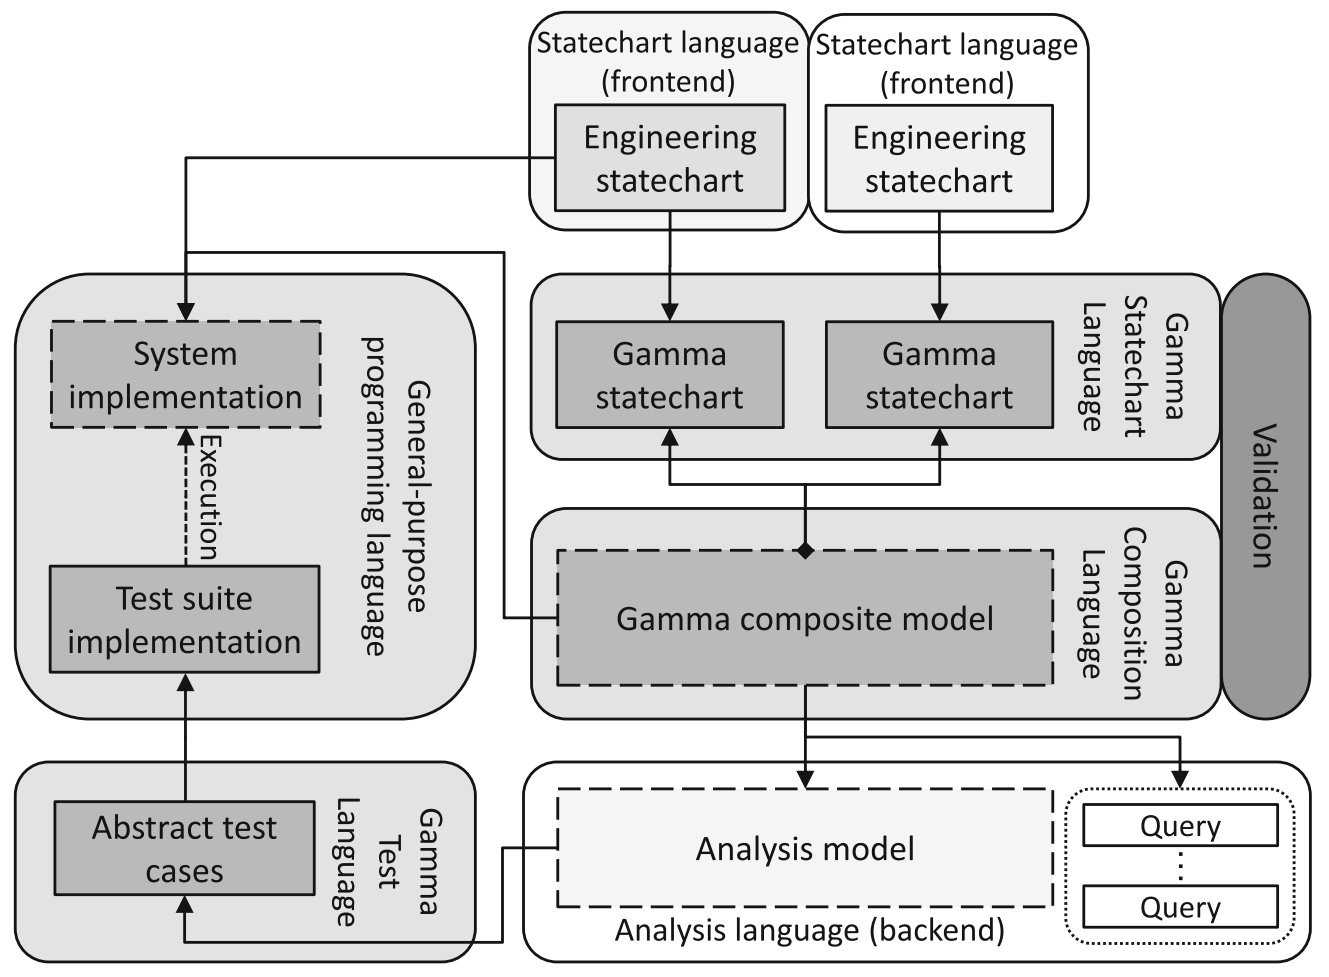
\includegraphics[width=0.8\textwidth, keepaspectratio]{figures/gamma.png}
\caption{The functionalities of the Gamma framework~\cite{Graics2020}.}
\label{fig:gamma}
\end{figure}

\subsection{Theta Model Checking Framework}\label{ssec:theta}

The Theta Model Checking Framework\footnote{\url{https://inf.mit.bme.hu/en/theta} and \url{https://github.com/ftsrg/theta}}~\cite{Theta} is a generic, modular, and configurable model checking framework. The architecture of Theta is shown in \autoref{fig:theta}.

\begin{figure}[htbp]
\centering
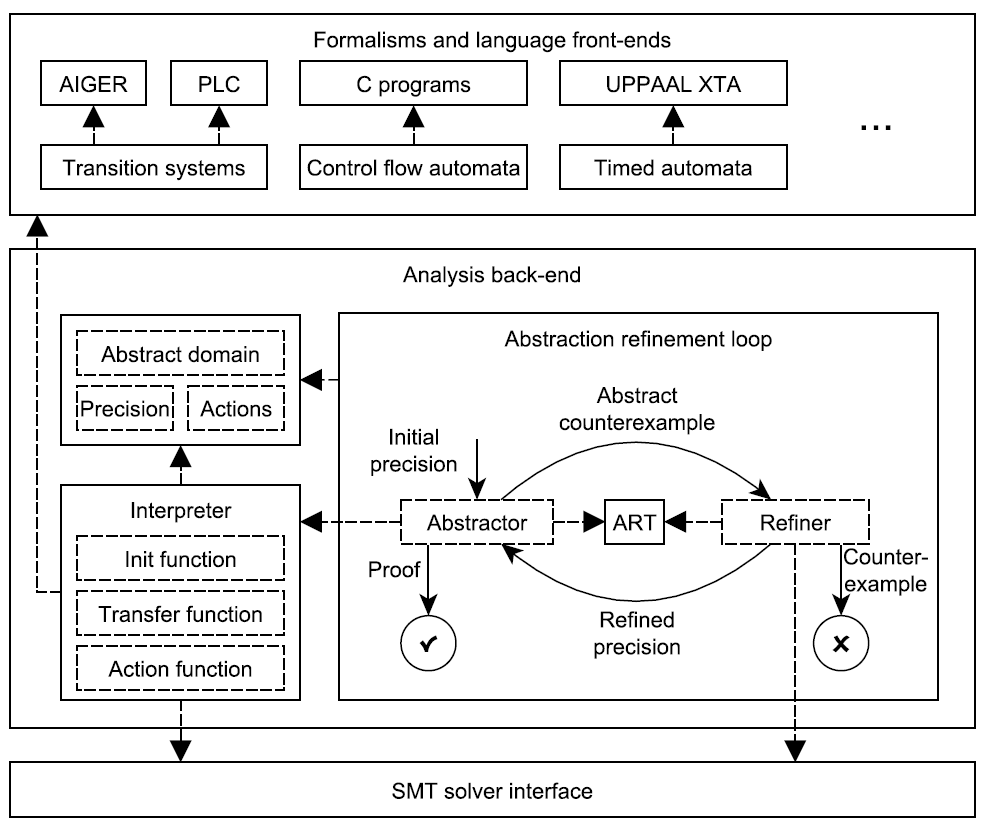
\includegraphics[width=0.8\textwidth, keepaspectratio]{figures/theta.png}
\caption{The architecture of the Theta framework~\cite{Theta}.}
\label{fig:theta}
\end{figure}

Theta can be divided into four main layers.

\begin{itemize}
    \item \textit{Formalisms}: Theta can handle multiple formalisms as input, such as \textit{timed automata}, \textit{control flow automata}, and \textit{transition systems}. Due to its modular architecture, further formalisms can be integrated. Every input model is transformed into a common inner abstract state space representation, regardless of the original input formalism. In this work, I focus on the \textit{Extended Symbolic Transition System} (XSTS)~\cite{XSTS} formalism as the input of Theta.
    \item \textit{Analysis back-end}: The analysis back-end provides the verification algorithms themselves. It contains formalism-specific \textit{interpreters} providing a common interface towards the algorithms by defining three functions: the \textit{init function} calculates the initial abstract states of the system, the \textit{transfer function} calculates the successor states of a given state, and the \textit{action function} calculates the available actions in a given abstract state. The verification algorithms usually use abstraction for which various \textit{abstract domains} are defined.
    \item \textit{SMT solver interface}: Many components rely on \textit{satisfiability modulo theories}~\cite{smt} (SMT) solvers for which a general interface is provided by Theta. It enables the use of different SMT solvers, and currently, it fully supports the Z3\footnote{\url{https://github.com/Z3Prover/z3}} solver developed by Microsoft.
    \item \textit{Tools}: Theta provides simple command-line applications which are responsible for reading the input and then instantiating and calling the algorithm specified by the arguments.
\end{itemize}

The analysis is done by the \textit{counterexample-guided abstraction refinement} (CEGAR) loop in the analysis back-end, Its central data structure is the \textit{abstract reachability graph}~\cite{theta-arg} (ARG) or \textit{abstract reachability tree} (ART). Its nodes represent abstract states, and its edges are labeled with actions. The ARG is modified by the two main parts of the loop, the \textit{abstractor} and the \textit{refiner}.

The initial ARG is constructed by the abstractor, based on the initial precision which comes from the selected algorithm and the formalism-specific interpreter. If there is no counterexample in the ARG, it \textit{proves} the correctness of the model. Otherwise, if an abstract counterexample exists, the refiner checks its feasibility. If the abstract counterexample is feasible, i.e., real, the model is incorrect, and the counterexample is returned. Otherwise, the refiner refines the abstraction of the ARG to eliminate that spurious counterexample.
